% \iffalse
\let\negmedspace\undefined
\let\negthickspace\undefined
\documentclass[beamer]{IEEEtran}
\usepackage{cite}
\usepackage{amsmath,amssymb,amsfonts,amsthm}
\usepackage{algorithmic}
\usepackage{graphicx}
\usepackage{textcomp}
\usepackage{xcolor}
\usepackage{txfonts}
\usepackage{listings}
\usepackage{enumitem}
\usepackage{mathtools}
\usepackage{gensymb}
\usepackage{comment}
\usepackage[breaklinks=true]{hyperref}
\usepackage{tkz-euclide} 
\usepackage{listings}
\usepackage{gvv}                                        
\def\inputGnumericTable{}                                 
\usepackage[latin1]{inputenc}                                
\usepackage{color}                                            
\usepackage{array}                                            
\usepackage{longtable}                                       
\usepackage{calc}                                             
\usepackage{multirow}                                         
\usepackage{hhline}                                           
\usepackage{ifthen}                                           
\usepackage{lscape}
\usepackage[export]{adjustbox}

\newtheorem{theorem}{Theorem}[section]
\newtheorem{problem}{Problem}
\newtheorem{proposition}{Proposition}[section]
\newtheorem{lemma}{Lemma}[section]
\newtheorem{corollary}[theorem]{Corollary}
\newtheorem{example}{Example}[section]
\newtheorem{definition}[problem]{Definition}
\newcommand{\BEQA}{\begin{eqnarray}}
\newcommand{\EEQA}{\end{eqnarray}}
\newcommand{\define}{\stackrel{\triangle}{=}}
\theoremstyle{remark}
\newtheorem{rem}{Remark}
\begin{document}
\parindent 0px
\bibliographystyle{IEEEtran}

\title{Assignment\\[1ex]11.15-23}
\author{ee23btech11215 - Penmetsa Srikar Varma$^{}$% <-this % stops a space
}
\maketitle
\newpage
\bigskip

\renewcommand{\thefigure}{\theenumi}
\renewcommand{\thetable}{\theenumi}
\section*{Question:}
Q23) A narrow sound pulse (for example, a short pip by a whistle) is sent across a
medium.\\\\ \brak{\text{a}} Does the pulse have a definite \brak{\text{i}} frequency, \brak{\text{ii}} wavelength, \brak{\text{iii}} speed
of propagation?\\\\ \brak{\text{b}} If the pulse rate is 1 after every 20 s, (that is the whistle is
blown for a split of second after every 20 s), Is the frequency of note produced
by whistle equal to 1/20 or 0.05 Hz ?
\section*{Solution:}
{\centering
Table of Parameters\\
}
\begin{table}[h]
    \centering
    \begin{tabular}{|c|c|}
        \hline
         Parameter & Name of Parameter  \\
        \hline
         $\nu_0$ & first harmonic \\
         \hline
          $\nu_n$ & $n^{th}$ harmonic \\
         \hline
         l & length of short pip \\
         \hline
         V & velocity of sound wave\\
         \hline
         $\lambda$ & wavelength of sound wave\\
         \hline
         A & amplitude of sound wave\\
         \hline
         x,y & co-ordinates of point on wave\\
         \hline
         k & wave number\\
         \hline
         $\omega$ & angular frequency of wave\\
         \hline
         t & time\\
         \hline
    \end{tabular}

    \label{tab:t1}
\end{table}

\brak{\text{a}} Let us assume, equation of sound pulse \brak{\text{in\ resonance}} produced in short pip and is given by:\\
\begin{align}
    \label{a1}
    \text{y}&=\text{A}\ \text{sin}\text{kx}\ \text{cos}\omega\text{t}
\end{align}
\begin{figure}[h]
    \centering
    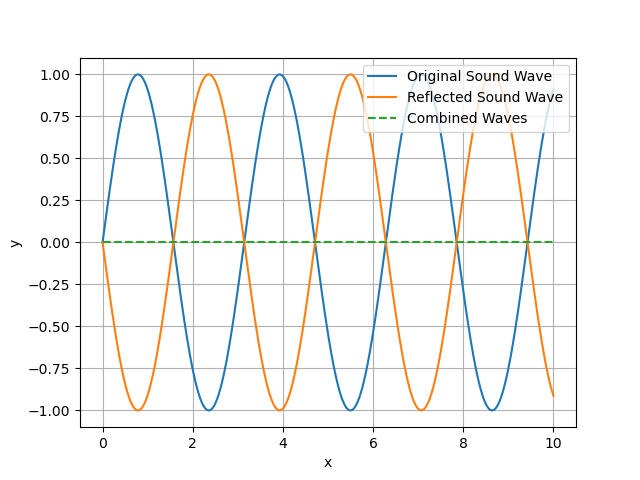
\includegraphics[scale=0.50]{ncert-physics/11/15/23/figs/py_w.png}
    \label{fig:enter-label}
\end{figure}

Hence from \brak{\ref{a1}} we know that,\\
if pip is closed at one end\\
\begin{align}
\label{a2}
\nu_\text{n}&=\text{n}\left(\frac{\text{V}}{\text{2L}}\right)\ \text{and}\ \text{l}=\text{n}\left(\frac{\lambda}{2}\right)
\end{align}
if pip is opened at both ends\\
\begin{align}
\label{a3}
\nu_\text{n}&=\brak{2\text{n}+1}\left(\frac{\text{V}}{4\text{L}}\right)\ \text{and}\ \text{l}=\brak{2\text{n}+1}\left(\frac{\lambda}{4}\right)
\end{align}
Therefore, from \brak{\ref{a2}} and \brak{\ref{a3}}\\\\
We can say that frequency $\nu_\text{n}$ and wavelength $\lambda$ of sound pulse in pip are not constant bu velocity V of sound pulse in pip is constant\\

\brak{\text{b}} And we know the relation that:
\begin{align}
    \label{a4}
    \nu_\text{n}&=\text{n}\left(\frac{\text{V}}{2\text{L}}\right)\ \text{or}\ \nu_\text{n}=\brak{2\text{n}+1}\left(\frac{\text{V}}{4\text{L}}\right)
\end{align}
Hence, The frequency of the note $\nu_n$ produced will not be equal to 0.05 Hz or $\frac{1}{20}$ Hz 

\end{document}
